\documentclass{standalone}
\usepackage[calc]{picture}
\usepackage{graphicx,transparent,color,amsmath,amssymb,amsfonts}
\graphicspath{Fig_INIT_subfigs}
\setlength{\unitlength}{1in}
\usepackage{helvet}
\renewcommand{\familydefault}{\sfdefault}
\begin{document}

% example frame 
\begin{picture}(6.45, 5.8)(0,-5.8)
% \linethickness{0.02in}
\put(0.2,-1.72){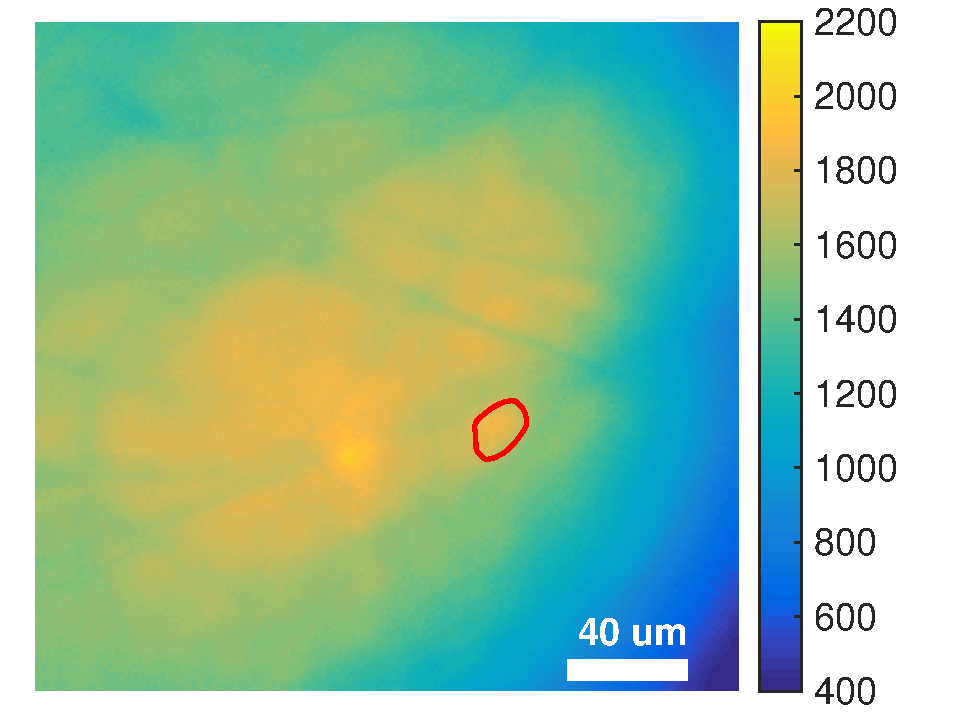
\includegraphics[height=1.5in]{Fig_INIT_subfigs/example_frame.pdf}}
\put(0.05, -0.2){\large\textbf{A}}
\put(0.85, -0.15){\small Raw data}

% mean neuron activity 
\put(2.3,-1.72){\includegraphics[height=1.5in]{Fig_INIT_subfigs/example_mean.pdf}}
\put(2.6, -0.17){\small{Mean cellular activity}}
\put(2.15, -0.2){\large\textbf{B}}

% correlation images 
\put(4.4,-1.72){\includegraphics[height=1.5in]{Fig_INIT_subfigs/example_Cn.pdf}}
\put(4.75, -0.15){\small{Correlation image}}
\put(4.25, -0.2){\large \textbf{C}}

%% example, single neuron 
% ground truth 
\put(0.25,-2.7){\includegraphics[height=0.7in]{Fig_INIT_subfigs/single_neuron_spatial.pdf}}
\put(0.25, -1.9){\small{True shape}}
\put(0.05, -1.95){\large\textbf{D}}
% filtered trace, single neuron 
\put(3.2,-2.75){\includegraphics[height=0.8in]{Fig_INIT_subfigs/single_neuron_temporal_filtered.pdf}}
\put(3.9, -1.9){\small{Filtered traces}}

% raw traces single neuron 
\put(1.0,-2.7){\includegraphics[height=0.8in]{Fig_INIT_subfigs/single_neuron_temporal_raw.pdf}}
\put(1.8, -1.9){\small{Raw traces}}

\put(5.55,-2.7){\includegraphics[height=0.7in]{Fig_INIT_subfigs/single_neuron_spatial_initialized.pdf}}
\put(6.3,-2.75){\color{black}\line(0,1){.8}}
\put(0.2,-2.75){\color{black}\line(1,0){6.1}}
\put(0.2,-2.75){\color{black}\line(0,1){.8}}
\put(0.2,-1.95){\color{black}\line(1,0){6.1}}
\put(5.55, -1.9){\small{Initialization}}


%% example, double neuron 
% ground truth 
\put(0.25,-3.7){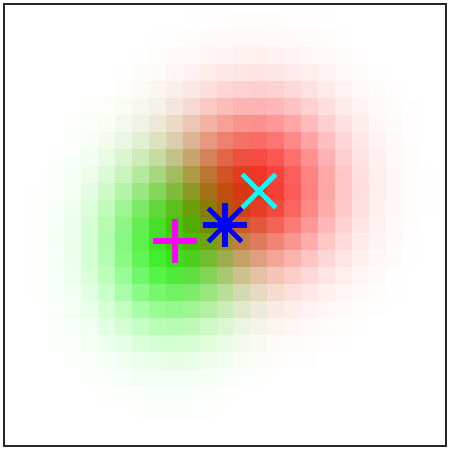
\includegraphics[height=0.7in]{Fig_INIT_subfigs/double_neuron_spatial.pdf}}
\put(0.25, -2.9){\small{True shape}}
\put(0.05, -2.95){\large\textbf{E}}
% filtered trace, dobule neuron 
\put(3.2,-3.75){\includegraphics[height=0.8in]{Fig_INIT_subfigs/double_neuron_temporal_filtered.pdf}}
\put(3.9, -2.9){\small{Filtered traces}}

% raw traces double neuron 
\put(1.0,-3.7){\includegraphics[height=0.8in]{Fig_INIT_subfigs/double_neuron_temporal_raw.pdf}}
\put(1.8, -2.9){\small{Raw traces}}


\put(5.55,-3.7){\includegraphics[height=0.7in]{Fig_INIT_subfigs/double_neuron_spatial_initialized.pdf}}
\put(5.55, -2.9){\small{Initialization}}
\put(6.3,-3.75){\color{black}\line(0,1){.8}}
\put(0.2,-3.75){\color{black}\line(1,0){6.1}}
\put(0.2,-3.75){\color{black}\line(0,1){.8}}
\put(0.2,-2.95){\color{black}\line(1,0){6.1}}

% detected neurons 
\put(0.2,-5.5){\includegraphics[height=1.5in]{Fig_INIT_subfigs/example_init.pdf}}
\put(0.65, -3.95){\small{Detected neurons}}
\put(0.05, -4.0){\large\textbf{F}}

\put(2.12,-5.75){\includegraphics[height=1.8in]{Fig_INIT_subfigs/example_init_similarity.pdf}}
\put(2.12, -4.0){\textbf{G}}
\put(4.25,-5.75){\includegraphics[height=1.8in]{Fig_INIT_subfigs/example_min_cn_pnr.pdf}}
\put(4.25, -4.0){\textbf{H}}
\end{picture}
\end{document}
